Entropy, in essence, represents the minimal quantity of bits required to unequivocally distinguish an object within a set. Consequently, it serves as a foundational metric for the space utilization in compressed data representations. The ultimate aim of compressed data structures is to occupy space nearly equivalent to the entropy required for object identification, while simultaneously enabling efficient querying operations. This pursuit lies at the core of optimizing data compression techniques: achieving a balance between storage efficiency and query responsiveness. \vspace{0.4cm}

\noindent There are plenty of compression techniques, yet they share certain fundamental steps. In Figure \ref{fig:typical_processes} is shown the typical processes employed for data compression. These procedures depend on the nature of the data, and the arrangement or fusion of the blocks in \ref{fig:typical_processes} may differ. Numerical manipulation, such as predictive coding and linear transformations, is commonly employed for waveform signals like images and audio. Logical manipulation involves altering the data into a format more feasible to compression, including techniques such as run-length encoding, zero-trees, set-partitioning information, and dictionary entries. Then, source modeling is used to predict the data's behavior and structure, which is crucial for entropy coding.

\begin{figure}[h]
    \centering
    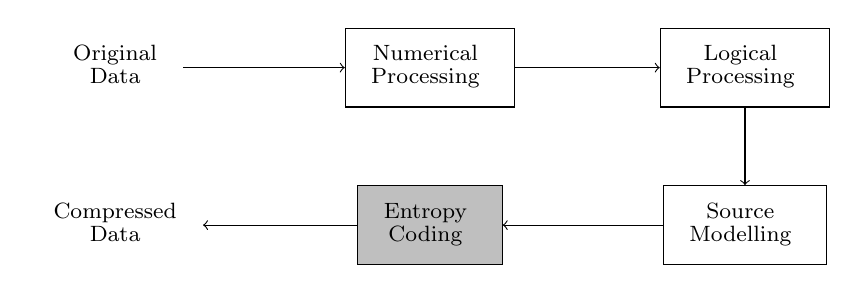
\begin{tikzpicture}
        \renewcommand{\arraystretch}{0.7} % Adjust line spacing in the tabular environment
        % Blocks
        \node (block1) at (0,0) {
            \begin{tabular}{c}
                \footnotesize Original \\
                \footnotesize Data
            \end{tabular}
        };
        \node[draw, minimum width=1cm, minimum height=1cm, align=center] (block2) at (4,0) {
            \begin{tabular}{c}
                \footnotesize Numerical \\
                \footnotesize Processing
            \end{tabular}
        };
        \node[draw, minimum width=1cm, minimum height=1cm, align=center] (block3) at (8,0) {
            \begin{tabular}{c}
                \footnotesize Logical \\
                \footnotesize Processing
            \end{tabular}
        };
        \node[draw, minimum width=1cm, minimum height=1cm, align=center] (block4) at (8,-2) {
            \begin{tabular}{c}
                \footnotesize Source \\
                \footnotesize Modelling
            \end{tabular}
        };
        \node[draw, minimum width=1cm, minimum height=1cm, align=center, fill=lightgray] (block5) at (4,-2) {
            \begin{tabular}{c}
                \footnotesize Entropy \\
                \footnotesize Coding
            \end{tabular}
        };
        \node (block6) at (0,-2) {
            \begin{tabular}{c}
                \footnotesize Compressed \\
                \footnotesize Data
            \end{tabular}
        };

        % Arrows
        \draw[->] (block1) -- (block2);
        \draw[->] (block2) -- (block3);
        \draw[->] (block3) -- (block4);
        \draw[->] (block4) -- (block5);
        \draw[->] (block5) -- (block6);


        % \draw[dotted, color=red] (block1.north west) -- (block3.north east) -- (block4.south east) -- (block4.south west) -- (block4.north west) -- (block6.north west) -- (block1.north west);

    \end{tikzpicture}
    \caption{Typical processes in data compression}\label{fig:typical_processes}
\end{figure}

\noindent These initial numerical and logical processing stages typically aim to transform the data, exploiting specific properties like signal correlation or symbol repetition, to create a representation with enhanced statistical redundancy (e.g., more frequent symbols, predictable patterns). A common feature among most compression systems is the incorporation of \emph{entropy coding} as the final process, wherein information is represented in the most compressed form possible. This stage may bear a significant impact on the overall compression ratio, as it is responsible for the final reduction in the data size. In this chapter we will delve into the principles of entropy coding, exploring the fundamental concepts and methods that underpin this crucial stage of data compression.

\section*{Worst Case Entropy}
In its simplest form, entropy can be seen as the minimum number of bits required by identifiers (\emph{codes}, see \autoref{sec:source_and_codes}), when each element of a set $U$ has a unique code of identical length. This is called the \emph{worst case entropy} of $U$ and it's denoted by $H_{wc}(U)$. The worst case entropy of a set $U$ is given by the formula:
\begin{equation}
    H_{wc}(U) =  \log |U|
\end{equation}
where $|U|$ is the number of elements in $U$.

\begin{remark}
    If we used codes of length $l < H_{wc} (U)$, we would have only $2^l \leq 2^{H_{wc}(U)} = |U|$ possible codes, which is not enough to uniquely identify all elements in $U$.
\end{remark}

\noindent The reason behind the attribute \emph{worst case} is that if all codes are of the same length, then this length must be at least $\lceil \log |U| \rceil$ bits to be able to uniquely identify all elements in $U$. If they all have different lengths, the longest code must be at least $\lceil \log |U| \rceil$ bits long.

% \begin{example}[Worst case entropy of $\mathcal{T}_n$]
%     Let $\mathcal{T}_n$ be the set of all general ordinal trees \cite{benoit2005representing} with $n$ nodes. In this case, each node has an arbitrary number of children and distinguishes their order. Given $n$ nodes, the number of possible ordinal trees its the (n-1)-th Catalan number, which is given by the formula:
%     \begin{equation}
%         |\mathcal{T}_n| = \frac{1}{n} \binom{2n -2}{n-1}
%     \end{equation}
%     By using the Stirling approximation, we can estimate the worst case entropy of $\mathcal{T}_n$ as:
%     \begin{equation*}
%         |\mathcal{T}_n| = \frac{(2n-2)!}{n!(n-1)!} = \frac{(2n-2)^{2n-2} e^n e^{n-1}}{e^{2n-2} n^n (n-1)^{n-1} \sqrt{\pi n}} \left(1+ \left(O\frac{1}{n}\right) \right)
%     \end{equation*}
%     That is equal to $\frac{4^n}{n^{3/2}} \cdot \Theta (1)$, therefore
%     \begin{equation}
%         H_{wc} (\mathcal{T}_n) = \log | \mathcal{T}_n | = 2n - \Theta(\log n)
%     \end{equation}
%     We have then found the minimum numbers of bits required to uniquely identify (\emph{encode}) a general ordinal tree with $n$ nodes.
% \end{example}
\begin{example}[Worst-case entropy of $\mathcal{T}_n$]
    Let $\mathcal{T}_n$ denote the set of all general ordinal trees \cite{benoit2005representing} with $n$ nodes. In this scenario, each node can have an arbitrary number of children, and their order is distinguished. With $n$ nodes, the number of possible ordinal trees is the $(n-1)$-th Catalan number, given by:
    \begin{equation}
        |\mathcal{T}_n| = \frac{1}{n} \binom{2n - 2}{n - 1}
    \end{equation}
    Using Stirling's approximation, we can estimate the worst-case entropy of $\mathcal{T}_n$ as:
    \begin{equation*}
        |\mathcal{T}_n| = \frac{(2n-2)!}{n!(n-1)!} = \frac{(2n-2)^{2n-2} e^n e^{n-1}}{e^{2n-2} n^n (n-1)^{n-1} \sqrt{\pi n}} \left(1+ O\left(\frac{1}{n}\right)\right)
    \end{equation*}
    This simplifies to $\frac{4^n}{n^{3/2}} \cdot \Theta (1)$, hence
    \begin{equation}
        H_{wc} (\mathcal{T}_n) = \log |\mathcal{T}_n| = 2n - \Theta(\log n)
    \end{equation}
    Thus, we have determined the minimum number of bits required to uniquely identify (encode) a general ordinal tree with $n$ nodes.
\end{example}
